\documentclass{article}
\usepackage[preprint]{nips_2018}
\usepackage{amsmath}
\usepackage{amsthm}
\usepackage{array}
\usepackage{booktabs}
\usepackage{graphicx}
\usepackage{wasysym}
\usepackage{tabularx}
\usepackage{threeparttable}
\usepackage[newfloat]{minted}
\usepackage{caption}
\usepackage{subcaption}
\usepackage{parcolumns}
\usepackage{booktabs}
\usepackage{enumerate}

% fix the default super-ugly coloured link boxes (citations, urls, figure numbers, footnote numbers, etc)
\usepackage[pagebackref=false,breaklinks=true,colorlinks,bookmarks=false,urlcolor=blue,linkcolor=blue,citecolor=blue]{hyperref}

\usepackage[utf8]{inputenc} % allow utf-8 input
\usepackage[T1]{fontenc}    % use 8-bit T1 fonts
\usepackage{hyperref}       % hyperlinks
\usepackage{url}            % simple URL typesetting
\usepackage{booktabs}       % professional-quality tables
\usepackage{amsfonts}       % blackboard math symbols
\usepackage{nicefrac}       % compact symbols for 1/2, etc.
\usepackage{microtype}      % microtypography

\usepackage{adjustbox}

\newcommand*\OK{\ding{51}}

\newcolumntype{R}[2]{%
  >{\adjustbox{angle=#1,lap=\width-(#2)}\bgroup}%
  l%
  <{\egroup}%
}
\newcommand*\rot{\multicolumn{1}{R{30}{2.0em}}}

\setlength{\textfloatsep}{0.1cm}

% \DeclareMathOperator requires \usepackage{amsmath}
\DeclareMathOperator*{\argmindown}{argmin}   % limit is placed underneath
\DeclareMathOperator{\argminright}{argmin}   % limit is placed on the right side
% more details:
% https://tex.stackexchange.com/questions/5223/command-for-argmin-or-argmax

\begin{document}

% TODO: title could possibly be improved
%\title{\texttt{ensmallen}: a generic C++ library for fast optimization}  %% it's not clear what "optimization" refers to here
%% other possibilities:
%\title{\texttt{ensmallen}: a flexible C++ library for function optimization in machine learning}
%\title{\texttt{ensmallen}: a fast C++ library for function optimization in machine learning}
%\title{\texttt{ensmallen}: a C++ library for fast function optimization in machine learning}
%\title{\texttt{ensmallen}: a C++ library for fast and flexible function optimization}
%\title{\texttt{ensmallen}: a C++ library of fast and flexible function optimizers}
%\title{\texttt{ensmallen}: a library of flexible function optimizers in C++}
%\title{\texttt{ensmallen}: a library of fast and flexible function optimizers in C++}
%\title{\texttt{ensmallen}: a flexible C++ library for function optimization}
\title{\texttt{ensmallen}: a flexible C++ library for efficient function optimization}

% Alphabetical ordering?
% TODO: check affiliations
\author{Shikhar Bhardwaj \\
Delhi Technological University \\
Delhi, India 110042 \\
\texttt{shikhar\_bt2k15@dtu.ac.in}
\And
Ryan R. Curtin \\
RelationalAI \\
Atlanta, GA, USA 30318 \\
\texttt{ryan@ratml.org}
\And
Marcus Edel \\
Free University of Berlin \\
Arnimallee 7, 14195 Berlin \\
\texttt{marcus.edel@fu-berlin.de}
\And
%% CS: I've added "Independent Researcher" below for now,
%% CS: as a blank affiliation looks weird and incomplete
Yannis Mentekidis \\
Independent Researcher \\
\texttt{mentekid@gmail.com}
% any affiliation/email?
%% CS: googling suggests that Yannis is/was affiliated with Aristotle University of Thessaloniki 
%% CS: and is perhaps now with Amazon
\And
%% CS: I have two affiliations, so I've listed them on two lines
Conrad Sanderson \\
Data61, CSIRO, Australia \\
University of Queensland, Australia\\
\texttt{conradsand@ieee.org}
}

\maketitle

\begin{abstract}
\vspace*{-0.3em}
%% the abstract below still needs more meat and sharpening
We present {\tt ensmallen}, a fast and flexible C++ library for mathematical optimization of 
arbitrary user-supplied functions,
which can be applied to many machine learning problems.
Several types of optimizations are supported, including differentiable,
separable, constrained, and categorical objective functions.
The library provides many pre-built optimizers
(including numerous variants of SGD and Quasi-Newton optimizers)
as well as a flexible framework for implementing new optimizers and objective functions.
Implementation of a new optimizer requires only one method
and a new objective function requires at most four C++ functions. 
This can aid in the quick implementation and prototyping of new machine learning algorithms.
Due to the use of C++ template metaprogramming, {\tt ensmallen} is able to
support compiler optimizations that provide fast runtimes.
Empirical comparisons show that {\tt ensmallen} is able to outperform other
optimization frameworks (such as Julia and SciPy), sometimes by large margins.
The library is distributed under the 3-clause BSD license and is ready for use
in production environments.
\end{abstract}

\section{Introduction}

Mathematical optimization is the workhorse of virtually all machine learning
algorithms.  For a given objective function $f(\cdot)$
(which may have a special structure or constraints),
almost all machine learning problems can be boiled down
to the following optimization form:
%
%\vspace*{-0.2em}
\begin{equation}
\argmindown_x f(x)
\end{equation}
\vspace*{-1.5em}

Optimization is often computationally intensive and may correspond
to most of the time taken to train a machine learning model.  For instance, the
training of deep neural networks is dominated by the optimization of the model
parameters on the data~\cite{schmidhuber2015deep}.
Even popular machine learning models such as logistic regression
have training times mostly dominated by an optimization procedure~\cite{kingma2015adam}.
% TODO: might be nice to have something kind of anecdotal like 'even new
% students to the field of machine learning quickly encounter optimization' and
% cite, e.g., Andrew Ng's coursera course or some ML textbook or similar
%% CS: i think we don't need to explore this too much; better to cut out all the
%% CS: fat and stick with concrete examples, instead of veering off on tangents
%
% or maybe just a note about how many optimization techniques get published at
% NIPS every year?
%% CS: NIPS is too self-referential here

The ubiquity of optimization in machine learning algorithms highlights the need
for robust and flexible implementations of optimization algorithms.
We present {\tt ensmallen}, a C++ optimization toolkit
that contains a wide variety of optimization techniques for many types of
objective functions.  Through the use of C++ template
metaprogramming~\cite{Abrahams_2004},
{\tt ensmallen} is able to generate efficient code that can help with the
demanding computational needs of many machine learning algorithms.

Although there are many existing machine learning optimization toolkits, few
are able to take explicit advantage of metaprogramming based code optimizations,
and few offer robust support for various types of objective functions.
For instance, deep learning
libraries like Caffe~\cite{jia2014caffe},
PyTorch~\cite{paszke2017automatic},
and TensorFlow~\cite{abadi2016tensorflow}
each contain a variety of optimization techniques.  However, these techniques are
limited to stochastic gradient descent (SGD) and SGD-like optimizers that
operate on small batches of data points at a time.  Other machine learning
libraries, such as {\tt scikit-learn}~\cite{pedregosa2011scikit}
contain optimization algorithms but not in a coherent or reusable framework.
Many programming languages have higher-level packages for
mathematical optimization.  For example, {\tt
scipy.optimize}~\cite{jones2014scipy},
is widely used in the Python community, and MATLAB's function optimization
support has been available and used for many decades.
However, these
implementations are often unsuitable for modern machine learning tasks---for
instance, computing the full gradient of the objective function may not be
feasible because there are too many data points.

In this paper, we describe the functionality of {\tt ensmallen} and the types of
problems that it can be applied to.  We discuss the mechanisms by which {\tt ensmallen} is
able to provide both computational efficiency and ease-of-use.
We show a few examples that use the library, as well as empirical performance comparisons
with other optimization libraries.

{\tt ensmallen} is open-source software licensed under the 3-clause BSD
license~\cite{Rosen_2004_full}, 
allowing unencumbered use in both open-source and proprietary projects.
It is available for download from \url{https://www.ensmallen.org}.
Armadillo~\cite{sanderson2016armadillo} is used for efficient linear algebra operations,
with optional interface to GPUs via NVBLAS~\cite{nvidia2015}.


\vspace*{-0.2em}
\section{Types of Objective Functions}
\vspace*{-0.6em}

\begin{table}[b!]
\vspace*{-1.0em}
\centering
\begin{adjustbox}{scale={0.95}{0.95}}
    \begin{tabular}{@{} cl*{7}c @{}}
%  \begin{tabular}{ccccccc}
        & & \multicolumn{7}{c}{} \\[0.6ex]
            % If there is any coherent framework at all, this is true.
        & & \rot{unified framework}
            % If there is any support for constrained optimization, this is
            % true.
          & \rot{constraints}
            % If the optimization framework can do mini-batch, this is true.
          & \rot{batches}
            % If I can implement any arbitrary function to be optimized, this is
            % true.
          & \rot{arbitrary functions}
            % If I can implement any new optimization technique to use, this is
            % true.
          & \rot{arbitrary optimizers}
            % If the framework could take advantage of when the gradient is
            % sparse, this is true.
          & \rot{sparse gradients}
            % If the framework can handle categorical/discrete variables for
            % optimization, this is true.
          & \rot{categorical} \\
        \cmidrule[1pt]{2-9}
        % It might be reasonable to say mlpack categorical support is only
        % partial, but I am not sure exactly where we draw the line.
        & {\tt ensmallen}            & \CIRCLE & \CIRCLE & \CIRCLE & \CIRCLE & \CIRCLE & \CIRCLE & \CIRCLE \\
        % The Shogun toolbox has a fairly nice framework, but it doesn't support
        % sparse gradients or categorical features.  It also does not appear to
        % support constraints.
        & Shogun \cite{sonnenburg2010shogun}             & \CIRCLE & - & \CIRCLE & \CIRCLE & \CIRCLE & - & -
\\
        % VW doesn't appear to have any framework whatsoever and the code is
        % awful, but it does support batches and categorical features.
        & Vowpal Wabbit \cite{Langford2007VW}      & - & - & \CIRCLE  & - & - & - &
\CIRCLE \\
        % TensorFlow has a few optimizers, but they are all SGD-related.  You
        % can write most objectives easily (but some very hard), and categorical
        % support might be possible but would not be easy.
        & TensorFlow \cite{abadi2016tensorflow}        & \CIRCLE & -  & \CIRCLE  & \LEFTcircle & - &
\LEFTcircle & -  \\
        % Caffe has a nice framework, but it's only for SGD-related optimizers.
        % I think I could write a new one, but it is not the easiest thing in
        % the world.
        & Caffe \cite{jia2014caffe}           & \CIRCLE & -  & \CIRCLE & \LEFTcircle & \LEFTcircle
& - & - \\
        % Keras is restricted to neural networks and SGD-like optimizers.  I
        % don't know that it is possible to easily write a new optimizer.
        & Keras \cite{chollet2015}            & \CIRCLE & -  & \CIRCLE & \LEFTcircle & \LEFTcircle
& - & - \\
        % sklearn has a few optimizer frameworks, but they are all in different
        % places and have somewhat different support.
        & scikit-learn \cite{pedregosa2011scikit}       & \LEFTcircle & - & \LEFTcircle  & \LEFTcircle & -
& - & - \\
        % scipy has some nice optimizer framework but it does not support
        % batches or some of the more complex functionality.  And you can't
        % write your own.
        & SciPy \cite{jones2014scipy}             & \CIRCLE & \CIRCLE  & -  & \CIRCLE & - & - & - \\
        % MATLAB is very similar to scipy.
        & MATLAB \cite{mathworks2017OTB}            & \CIRCLE & \CIRCLE & - & \CIRCLE & - & - & - \\
        % Optim.jl isn't the only Julia package for optimization, but it's the
        % one we compare against.
        & Julia ({\tt Optim.jl}) \cite{julia}         & \CIRCLE & - & - & \CIRCLE & - & - & - \\
        \cmidrule[1pt]{2-9}
    \end{tabular}
\end{adjustbox}
%   \begin{tablenotes}\footnotesize
\caption{\footnotesize{
Feature comparison: \CIRCLE = provides feature,
\LEFTcircle = partially provides feature, - = does not provide feature.
{\it unified framework} indicates if there is some kind of generic/unified
optimization framework; {\it constraints} and {\it batches} indicate support for
constrained problems and batches; {\it arbitrary functions} means arbitrary
objective functions are easily implemented; {\it arbitrary optimizers} means
arbitrary optimizers are easily implemented; {\it sparse gradient} indicates
that the framework can natively take advantage of sparse gradients; and
{\it categorical} refers to if support for categorical features exists.
}}
\label{tab:functionality}
\vspace*{-1.8em}
\end{table}

{\tt ensmallen} provides a {\bf set of optimizers} for
optimizing {\bf user-defined objective functions}.  It is also easy to implement a
new optimizer in the {\tt ensmallen} framework.  Overall, our goal is to provide
an easy-to-use library that can solve the problem
%\vspace*{-0.4em}
%\begin{equation}
$\argminright_{x} f(x)$
%\end{equation}
%\vspace*{-0.4em}
%\noindent
for any function $f(x)$ that takes a vector or matrix input $x$.
In most cases, $f(x)$ will have special structure; one example might be that
$f(x)$ is differentiable.  Therefore, the abstraction we have designed for {\tt
ensmallen} can optionally take advantage of this structure.  For example, in
addition to $f(x)$, a user can provide an implementation of $f'(x)$, which in
turn allows first-order gradient-based optimizers to be used.  This generally
leads to significant speedups.


%% TODO: moving the list of optimizers here would improve the flow 
%% TODO: and free up a bit of space


Therefore, users may implement objective functions with specific properties that
the library can use to accelerate the computation.  These non-exclusive
properties are listed below:

\vspace*{-0.3em}
\begin{itemize} \itemsep -1pt
  \item {\bf arbitrary}: no assumptions can be made on $f(x)$
  \item {\bf differentiable}: $f(x)$ has a computable gradient $f'(x)$
  \item {\bf separable}: $f(x)$ is a sum of individual components: $f(x) =
\sum_{i} f_i(x)$
  \item {\bf categorical}: $x$ contains elements that can only take discrete
values
  %\item {\bf numeric}: all elements of $x$ take values in $\mathcal{R}$
  \item {\bf sparse}: the gradient $f'(x)$ or $f_i(x)$ (for a separable
function) is sparse
  \item {\bf partially differentiable}: the gradient $f'_j(x)$ is computable for
individual elements $x_j$ of $x$
  \item {\bf bounded}: $x$ is limited in the values that it can take
\end{itemize}
\vspace*{-0.3em}

Due to its straightforward abstraction framework, {\tt ensmallen} is able to
provide a large set of diverse optimization algorithms for objective functions
with these properties.  Below is a list of currently available optimizers:

% I guess to save some space we should group them.
%% CS: should we add citations to some (or all) of the listed optimisers?
%% CS: the MLSYS CFP states that "papers can be up to 6 pages (not including references)",
%% CS: so technically we can have 10000+ references.
\vspace*{-0.4em}
\begin{enumerate}[{~~~$\bullet$}]
\small
  \item {\bf SGD variants:}
      Stochastic Gradient Descent (SGD),
      SGD with Restarts,
      Parallel SGD (Hogwild!),
      Stochastic Coordinate Descent, 
      SMORMS3, AdaGrad,
      AdaDelta, RMSProp, Adam, AdaMax

  \item {\bf Quasi-Newton variants:} Limited-memory BFGS (L-BFGS), incremental
        Quasi-Newton method, Augmented Lagrangian Method

  \item {\bf Genetic variants:} Conventional Neuro-evolution, Covariance
        Matrix Adaptation Evolution Strategy

  \item {\bf Other:} Conditional Gradient Descent, Frank-Wolfe algorithm, Simulated Annealing

% These were a part of mlpack but not ensmallen.
  %\item {\bf Objective functions:} Neural Networks, Logistic regression,
  %    Matrix completion, Neighborhood Components Analysis, Regularized SVD,
  %    Reinforcement learning, Softmax regression, Sparse autoencoders,
  %    Sparse SVM
\end{enumerate}

In {\tt ensmallen}'s framework, if a user wants to optimize a differentiable objective
function, they only need to provide implementations of $f(x)$ and $f'(x)$, and
then they can use any of the gradient-based optimizers that {\tt ensmallen}
provides.  Table~\ref{tab:functionality} contrasts 
the classes of objective functions that can be handled by {\tt ensmallen}
and other popular frameworks and libraries.

Not every optimization algorithm provided by {\tt ensmallen} can be
used by every class of objective function; for instance, a gradient-based
optimizer such as L-BFGS cannot operate on a non-differentiable objective
function.
As such, the best the library can attain is to maximize the flexibility
available, so that a user can easily implement a function $f(x)$ and have it
work with as many optimizers as possible.

To accomplish the flexibility, {\tt ensmallen} makes heavy use of
C++ template metaprogramming.
When implementing an objective function to be optimized,
a user may only need to implement a few methods; metaprogramming is then automatically
used to check that the given functions match the requirements of the
optimizer that is being used.  When implementing an optimizer, we can assume
that the given function to be optimized meets the required assumptions of the
optimizers, and encode those requirements as compile-time checks
(via \texttt{\small static\_assert}).

For the most common case of a differentiable $f(x)$, the user only needs to
implement two methods:

\vspace*{-0.3em}
\begin{itemize} \itemsep -1pt
  \item \texttt{\small double Evaluate($x$)}: given coordinates $x$, this function
returns the value of $f(x)$.
  \item \texttt{\small void Gradient($x$, $g$)}: given coordinates $x$ and a reference
to $g$, set $g = f'(x)$.
\end{itemize}
\vspace*{-0.3em}

Alternatively, the user can simply implement a \texttt{\small EvaluateWithGradient()}
function that computes both $f(x)$ and $f'(x)$ simultaneously, which is useful
in cases where both the objective and gradient depend on similar computations.

The required API for separable differentiable objective functions (i.e.~those
that would use an optimizer like SGD) is very similar, except that
\texttt{\small Evaluate()}, \texttt{\small Gradient()} and \texttt{\small EvaluateWithGradient()}
should operate only on mini-batches, and utility methods \texttt{\small Shuffle()} and
\texttt{\small NumFunctions()} must be added.  The same pattern applies for other
types of objective functions: only a few methods specific to class of objective
function itself must be implemented and then any optimizer may be used.

\vspace*{-0.3em}
\section{Example: Learning Linear Regression Models}
\label{sec:linreg_example}
\vspace*{-0.5em}

As an example of usage, consider the linear regression objective
function\footnote{For simplicity, we ignore the bias term.  It can be
rederived by taking $x^*_i = (x_i, 1)$.}.  Given a dataset $X \in
\mathcal{R}^{n \times d}$ and associated responses $y \in \mathcal{R}^n$, the
model of linear regression is to assume that $y_i = x_i \theta$ for each
point and response $(x_i, y_i)$.  To fit this model $\theta \in \mathcal{R}^d$
to the data, we must find

%% CS: i've added \nolimits to save a bit of space
\vspace*{-1.1em}
\begin{equation}
\argmindown_\theta f(\theta) =   %% CS: for clarity
\argmindown_\theta \sum\nolimits_{i = 1}^n (y_i - x_i \theta)^2 =
\argmindown_\theta \| y - X \theta \|_F^2.
\end{equation}
\vspace*{-1.1em}

The objective function $f(\theta)$ has the associated gradient

\vspace*{-1.1em}
\begin{equation}
f'(\theta) = \sum\nolimits_{i = 1}^n -2 x_i (y_i - x_i \theta) = -2 X^T (y - X \theta).
\end{equation}
\vspace*{-1.1em}

We can implement these two functions in a class named {\tt LinearRegressionFunction},
as shown in Fig.~\ref{fig:LinearRegressionFunction}.
This is the entire required implementation to optimize the linear regression model with
any of the gradient-based optimizers in {\tt ensmallen}.

\begin{figure}[!tb]
\hrule\vspace*{0.5ex}
\begin{adjustbox}{scale={0.95}{0.90}}
\begin{minipage}{\textwidth}
\begin{minted}[fontsize=\small]{c++}
class LinearRegressionFunction {
 public:
  // Construct the LinearRegressionFunction with the given data
  LinearRegressionFunction(arma::mat& X_in, arma::vec& y_in) : X(X_in), y(y_in) {}

  // Compute the objective function
  double Evaluate(const arma::mat& theta) {
    return std::pow(arma::norm(y - X * theta), 2.0);
  }
  // Compute the gradient and store in 'gradient'
  void Gradient(const arma::mat& theta, arma::mat& gradient) {
    gradient = -2 * X.t() * (y - X * theta);
  }
 private:
  arma::mat& X; arma::vec& y;
};
\end{minted}
\end{minipage}
\end{adjustbox}
\vspace*{0.5ex}\hrule\vspace*{0.5ex}
\caption
  {
  Implementation of objective and gradient functions for linear regression,
  used by optimizers in \texttt{ensmallen}.
  The types {\footnotesize\tt arma::mat} and {\footnotesize\tt arma::vec}
  are matrix and vector types
  from Armadillo~\cite{sanderson2016armadillo}.
  }
\label{fig:LinearRegressionFunction}
\end{figure}

Given the user-defined {\tt LinearRegressionFunction} class,
the code snippet below
shows how the L-BFGS optimizer can be used to find the best parameters $\theta$:

\vspace*{-0.4em}
\begin{minted}[fontsize=\small]{c++}
    LinearRegressionFunction lrf(X, y); // we assume X and y already hold data
    ens::L_BFGS lbfgs; // create L-BFGS optimizer with default parameters

    arma::vec theta(X.n_rows, arma::fill::randu); // random uniform initialization
    lbfgs.Optimize(lrf, theta); // after this call, theta holds the solution
\end{minted}
\vspace*{-0.4em}

To use the small-batch SGD-like optimizers provided by {\tt ensmallen},
only a slight variation on the signature of \texttt{\small Evaluate()} and
\texttt{\small Gradient()} would be needed.

\vspace*{-0.3em}
\section{Automatic Metaprogramming for Ease of Use and Efficiency}
\vspace*{-0.5em}

When optimizing a given function $f(x)$, the computation of
the objective function $f(x)$ and its derivative $f'(x)$ often involve the
computation of identical intermediate results.  Consider the linear regression
objective function described
in Section~\ref{sec:linreg_example}, {\small $f(\theta) = \| y - X\theta \|_F^2$}.
For this objective function, the derivative $f'(\theta)$ has a related form of
{\small $-2 X^T (y -X \theta)$}.  Both the objective function and the derivative 
depend on the computation of the vector term {\small $(y - X \theta)$},
which can be computationally expensive to compute if $X$ is a large matrix.
Existing optimization frameworks do not have an easy way to avoid
this duplicate computation. In many cases, an optimization algorithm
may need the values of both $f(\theta)$ and $f'(\theta)$ for a given $\theta$.

Using template metaprogramming, {\tt ensmallen} provides an easy (and
optional) way for users to avoid this extra computational overhead.  Instead of
specifying individual \texttt{\small Evaluate()} and \texttt{\small Gradient()} functions, a user
may simply write an \texttt{\small EvaluateWithGradient()} function that returns both the
objective value and the gradient value for an input $\theta$.  As an example,
for the 
\texttt{LinearRegressionFunction} class in Fig.~\ref{fig:LinearRegressionFunction},
we can replace \texttt{\small Evaluate()} and \texttt{\small Gradient()}
with an implementation of \texttt{\small EvaluateWithGradient()}
that only computes $(y - X \theta)$ once:

\vspace*{-0.5em}
\begin{minted}[fontsize=\small]{c++}
    double EvaluateWithGradient(const arma::mat& theta, arma::mat& gradient) {
      const arma::vec v = (y - X * theta); // Cache result
      gradient = -2 * X.t() * v;  // Store gradient in the provided matrix
      return arma::accu(v % v); // Take squared norm of v
    }
\end{minted}
\vspace*{-0.5em}

% This is up here so that it's on the right page...
\begin{table}[t]
\begin{center}
\begin{tabular}{lcccc}
\toprule
 & {\tt ensmallen} & {\tt scipy} & {\tt Optim.jl} & {\tt samin} \\
\midrule
% TODO: these are just single-run results from Marcus' laptop!  We need to do
% 10 and average.
default & {\bf 0.004s} & 1.044s & 0.021s & 2.920s \\
tuned & & 0.5s-ish? & & ?? \\ % TODO
\bottomrule
\end{tabular}
\end{center}
\caption{Runtimes for $100000$ iterations of simulated annealing with different
frameworks on the simple Rosenbrock function.  Julia code runs do not count
compilation time.  The {\it tuned} row indicates that the code was manually
modified for speed.}
\label{tab:rosenbrock_results}
\end{table}

Template metaprogramming techniques are automatically used to
detect which methods exist, and a wrapper class will use suitable mix-ins in
order to provide any `missing` functionality~\cite{smaragdakis2000mixin}.  For
instance, if \texttt{\small EvaluateWithGradient()} is not provided, a version will be
automatically generated that calls both \texttt{\small Gradient()} and \texttt{\small Evaluate()} in turn.
Similarly, if \texttt{\small Evaluate()} or \texttt{\small Gradient()} does not exist, then {\tt
EvaluateWithGradient()} is called, and the unnecessary part of the result will
be discarded.

The use of template metaprogramming in this manner also allows for compiler optimizations that
would not otherwise be possible (and that are often not possible in other
frameworks).  Firstly, because the objective function class itself is a template
parameter, the compiler is able to avoid the overhead of a function pointer
dereference, which would not be easily possible when using a language with
virtual inheritance.  The compiler is also able to use inlining and any
optimizations that may imply, including removing temporary values and dead code
elimination.  Further, if {\tt ensmallen} automatically generates an
\texttt{\small Evaluate()} or \texttt{\small Gradient()} method from a user-supplied
\texttt{\small EvaluateWithGradient()} method, the compiler can in some cases recognize and
remove the computation of unnecessary results.  For instance, in an
automatically generated \texttt{\small Evaluate()} method, the computation of the gradient
from \texttt{\small EvaluateWithGradient()} can be avoided entirely.

Overall, the automatic code generation functionality in {\tt ensmallen}
reduces the requirements for users
when they are implementing their own objective functions to be optimized,
and allows users a way to provide more efficient implementations of their
objective functions.
This leads to quicker development, quicker results, and reduces the likelihood of bugs.

At the time of writing, the automatic code generation
is implemented for the most commonly-used cases:
full-batch and small-batch \texttt{\small Evaluate()}, \texttt{\small Gradient()},
and \texttt{\small EvaluateWithGradient()}.  We aim to expand this support to other
sets of methods for other types of objective functions.

% TODO: anything to write about the visualization page that we had set up?

\vspace*{-0.3em}
\section{Experiments}
\vspace*{-0.5em}

To demonstrate the benefits of the metaprogramming based code optimizations
that {\tt ensmallen} can exploit,
we compare the performance of {\tt ensmallen} with several other
optimization frameworks, including some that use automatic differentiation.

For our first experiment, we consider the simple and popular Rosenbrock
function~\cite{Rosenbrock1960}: $f([x_1, x_2]) = 100 (x_2 - x_1^2)^2 + (1 -
x_1^2)$.  For the optimizer, we use simulated
annealing~\cite{kirkpatrick1983optimization}, a gradient-free optimizer.
Simulated annealing will call the objective function numerous times; for each
simulation we limit the optimizer to 100k objective evaluations.  Since the
objective function is straightforward and is called many times, this can help us
understand the overheads of various frameworks.  We compare four frameworks%
%
\footnote{Another option here might be {\tt simulannealbnd()} 
in the Global Optimization Toolkit for MATLAB.
However, no license was available for these simulations.}
%
for this task:

\vspace*{-0.3em}
\begin{itemize}
\renewcommand{\itemsep}{-0.5ex}
  \item {\tt ensmallen}
  \item {\tt scipy.optimize.anneal}, from scipy 0.14.1~\cite{jones2014scipy}
  \item simulated annealing implementation in {\tt Optim.jl} with Julia
1.0.1~\cite{mogensen2018optim}
  \item {\tt samin} in the {\tt optim} package for GNU Octave~\cite{octave}
\end{itemize}
\vspace*{-0.3em}

% TODO: get Marcus' system specs.
We implemented and ran our code on a {\tt \$COMPUTER} running an {\tt
\$OPERATING\_SYSTEM} with gcc version {\tt \$GCC\_VERSION}, Julia version {\tt
\$JULIA\_VERSION}, Python {\tt \$PYTHON\_VERSION}, and Octave {\tt
\$OCTAVE\_VERSION}.

Initially, we implemented these functions as simply as possible and ran them
without any tuning, which reflects how a normal user might interact with the
software.  These results are seen in the first row of
Table~\ref{tab:rosenbrock_results}.  Only Julia and {\tt
ensmallen} are compiled, and thus are able to avoid the function pointer
dereference and take advantage of inlining and related optimizations.

%% CS: i'm not convinced that this conjecture is barking up the right tree;
%% CS: SciPy is in Python, which is by default an interpreted language.
%% CS: the slowdown many have nothing to do with inlining and simply due to
%% CS: Python being slow in general.
%% CS: it's possible to use PyPy or Numba to speed things up,
%% CS: in order to provide a "fairer" comparison against compiled languages.
%% CS: Octave also has an optional JIT compiler, which last time I checked
%% CS: needs to be explicitly enabled.
%% 
%% CS: i would suggest to stay away from the "we do inlining" argument,
%% CS: as it can be blown up too easily.
%% CS: furthermore, I would suggest to mention PyPy and/or Numba and Octave JIT
%% CS: (in order to show that we've done our homework),
%% CS: and then state something along the lines of
%% CS: "these approaches are not being used as we're comparing out-of-the-box performance"

% RC: agree, hopefully the paragraph below pushes this in more of a right
% direction.

However, both Python and GNU Octave have routes for acceleration, such as
numba~\cite{TODO} and MEX bindings for Octave/MATLAB.  Therefore, we hand-optimized the
Rosenbrock implementation using numba and ran the Octave implementation with the
JIT.  For the numba implementation, the underlying {\tt anneal.anneal()}
function had to be significantly modified.  These did produce some acceleration,
as can be seen in the second row of Table~\ref{tab:rosenbrock_results}.  For
Octave, a MEX binding did not produce a noticeable difference.

Next, we consider the linear regression example described in Sec.~\ref{sec:linreg_example}.
For this task we use the first-order L-BFGS optimizer~\cite{zhu1997algorithm}.
For {\tt ensmallen} we have 2 versions:
(i)~with only \texttt{\small EvaluateWithGradient()},
and
(ii)~with \texttt{\small Evaluate()} and \texttt{\small Gradient()}.
The code for these functions is as shown earlier.
For Julia we have the options of using manually defined objective and gradient functions,
or the gradient function can be automatically computed by 
{\tt Calculus.jl}
({\href{https://github.com/JuliaMath/Calculus.jl}{\footnotesize github.com/JuliaMath/Calculus.jl})
or {\tt ForwardDiff.jl}~\cite{RevelsLubinPapamarkou2016}.
Overall we compare across the following:

\vspace*{-0.3em}
\begin{itemize}
\renewcommand{\itemsep}{-0.5ex}
  \item {\tt ensmallen}-1: only \texttt{\small EvaluateWithGradient()} implemented
  \item {\tt ensmallen}-2: both \texttt{\small Evaluate()} and \texttt{\small Gradient()} separately
implemented
  \item {\tt Calculus.jl}: uses the default {\tt Calculus.jl} for
computing the gradient with {\tt Optim.jl}
  \item {\tt ForwardDiff.jl}: uses {\tt ForwardDiff.jl} for computing
the gradient with {\tt Optim.jl}
  \item {\tt Optim.jl}: implements the gradient manually
  \item {\tt scipy}: implements both objective and
gradient
  \item {\tt bfgsmin}: uses {\tt optim} package for GNU Octave
\end{itemize}
\vspace*{-0.3em}

Results for various data sizes are shown in Table~\ref{tab:lbfgs}.  For each
implementation, L-BFGS was allowed to run for only $10$ iterations and never
converged in fewer iterations.  The datasets used for training are highly noisy random
data with a slight linear pattern. Note that the exact data is not relevant
for the experiments here, only its size.  Runtimes are reported as the
average across 10 runs.

\begin{table}
\begin{center}
\begin{tabular}{lccccc}
\toprule
{\em algorithm} & $d$: 100, $n$: 1k & $d$: 100, $n$: 10k & $d$: 100, $n$:
100k & $d$: 1k, $n$: 100k \\
\midrule
% TODO: this was only one trial on Ryan's desktop!
{\tt ensmallen}-1 & {\bf 0.001s} & {\bf 0.006s} & {\bf 0.139s} & {\bf 1.698s} \\
{\tt ensmallen}-2 & 0.002s & 0.008s & 0.204s & 2.497s \\
{\tt Calculus.jl} & 0.172s & 0.960s & 27.428s & 2535.507s \\
{\tt ForwardDiff.jl} & 0.553s & 1.162s & 6.665s & 778.250s \\
{\tt Optim.jl} & 0.007s & 0.025s & 0.390s & 4.107s \\
{\tt scipy.optimize} & 0.002s & 0.010s & 0.198s & 2.022s \\
{\tt bfgsmin} & 0.215s & 1.705s & 15.998s & ??? \\
\bottomrule
\end{tabular}
\end{center}
\caption{Runtimes for linear regression function with various dataset sizes,
with $n$ indicating the number of samples,
and $d$ indicating the dimensionality of each sample.
All Julia runs do not count compilation time.}
\label{tab:lbfgs}
\end{table}

The results indicate that {\tt ensmallen} with \texttt{\small EvaluateWithGradient()}
is the fastest approach.
Furthremore, the use of \texttt{\small EvaluateWithGradient()} yields considerable
speedup of almost 1.5x over the {\tt ensmallen} implementation with both the
objective and gradient implemented separately.  In addition, although the
automatic differentiation support makes it easier for users to write their
code, it is clear that the code generated by the automatic differentiators
({\tt Calculus.jl} and {\tt ForwardDiff.jl})
is far from optimal, with runs that are slower by up to three orders of magnitude.

% TODO: show flexibility of optimization with learning curves:
%  - use LinearRegressionFunction modified for small batches
%  - make sure Info or Debug output is on
%  - run with a whole boatload of SGD variants
%  - parse the output with awk/sed into a csv of objectives per epoch
%  - plot it
%  - profit!
%
% Probably a snippet showing the actual code to run with a bunch of different
% optimizers is good too.  Other things can be cut to make space.

Lastly, we demonstrate the easy pluggability in {\tt ensmallen}
for using various optimizers on the same task.
Using a version of \texttt{\small LinearRegressionFunction} from Sec.~\ref{sec:linreg_example}
adapted for separable differentiable optimizers,
we run six optimizers with default parameters in just 7 lines of code,
as shown in Fig.~\ref{fig:learning_curve}(a).
Applying these optimizers to the {\tt YearPredictionMSD}
dataset from the UCI repository~\cite{ucimlrepository} % TODO: add to bibtex
yields the learning curves shown in Fig.~\ref{fig:learning_curve}(b).
Any other optimizers for separable differentiable objective
functions can be dropped into place in the same manner.

% This facilitates the evaluation of various optimizers
% for user-defined objective functions.

\begin{figure}[h!]
\begin{minipage}[t]{1\textwidth}
\begin{adjustbox}{scale={0.90}{0.90}}
\begin{minipage}{0.50\textwidth}
\centering
\begin{minted}[fontsize=\footnotesize]{c++}
// X and y are data
LinearRegressionFunction lrf(X, y);

ens::StandardSGD<>().Optimize(lrf, sgdModel);
ens::Adam().Optimize(lrf, adamModel);
ens::AdaGrad().Optimize(lrf, adagradModel);
ens::SMORMS3().Optimize(lrf, smorms3Model);
ens::SPALeRASGD().Optimize(lrf, spaleraModel);
ens::RMSProp().Optimize(lrf, rmspropModel);
\end{minted}
\end{minipage}
\end{adjustbox}
\hfill
\begin{minipage}{0.49\textwidth}
  \centering
  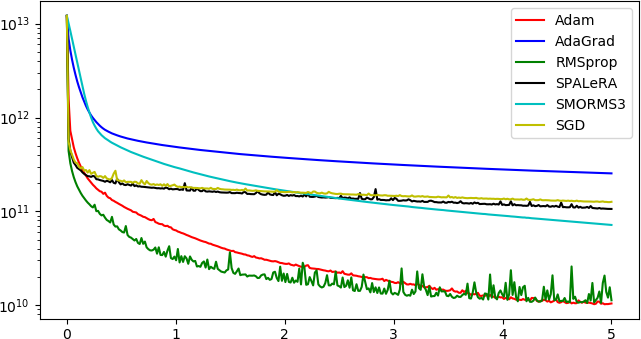
\includegraphics[width=\textwidth,height=0.45\textwidth]{experiments/learning_curves_crop.png}
\end{minipage}
\end{minipage}
\begin{minipage}[t]{1\textwidth}
\begin{minipage}{0.50\textwidth}
\centering
(a)
\end{minipage}
\hfill
\begin{minipage}{0.49\textwidth}
\centering
(b)
\end{minipage}
\end{minipage}
\caption
  {
  (a): example code for using 
  six {\tt ensmallen} optimizers with default parameters
  to optimize a linear regression function;
  (b): corresponding learning curves
  on the {\tt YearPredictionMSD} dataset~\cite{ucimlrepository}
  over 5 epochs of training.
  The optimizers can be tuned for better performance.
  }
\label{fig:learning_curve}
\end{figure}

\vspace*{-0.3em}
\section{Conclusion}
\vspace*{-0.5em}

We have described {\tt ensmallen}, a flexible C++ library for function
optimization that provides an easy interface for users to implement and optimize
their desired objective functions.  Many types of functions can be optimized,
including separable and constrained functions.  The library is fast due to its
use of template metaprogramming and the Armadillo matrix library for linear
algebra.  In addition, template metaprogramming is used to make user
implementation easier by automatically generating missing methods.

The library provides many pre-built optimizers (including numerous variants
of SGD and Quasi-Newton optimizers).
We aim to expand the library with further optimization techniques
as the need arises.  Since {\tt ensmallen} is open source,
external contributions to the codebase are welcome.

% GPU support for optimization is available either through the use of the NVBLAS
% library~\cite{nvidia2015} or the forthcoming Bandicoot C++ GPU matrix library.
%% Conrad: is it ok if we mention that here?  It's a really nice selling point
%% and I am sure at least one reviewer will be thinking about GPUs.

%% CS: we don't have much room, so I moved the mention of NVBLAS to the intro.
%% CS: i think it flows better there.
%% CS: mentioning it here in the conclusion seems a bit left-field.
%% CS: we also don't have a good reference for Bandicoot yet


{\tt ensmallen} is already in use as the optimization toolkit of the {\tt
mlpack} machine learning library~\cite{mlpack2018}.  For more information on the
toolkit, see the website and documentation at \url{https://www.ensmallen.org/}.

%\begin{small}
{\bf Acknowledgements.}
We would like to thank the many contributors to {\tt ensmallen},
who are listed on the associated website.
%\end{small}

% \subsubsection*{Acknowledgements}
% \vspace*{-0.5em}
% 
% The development team of {\tt ensmallen} does not include just the authors named
% here but also a long list of other contributors.  See
% \url{https://www.ensmallen.org/about.html} for more information.
% % TODO: that URL may change



\bibliographystyle{plain}
\bibliography{paper}

\end{document}
